\begin{figure*}[!htbp]
    \centering
    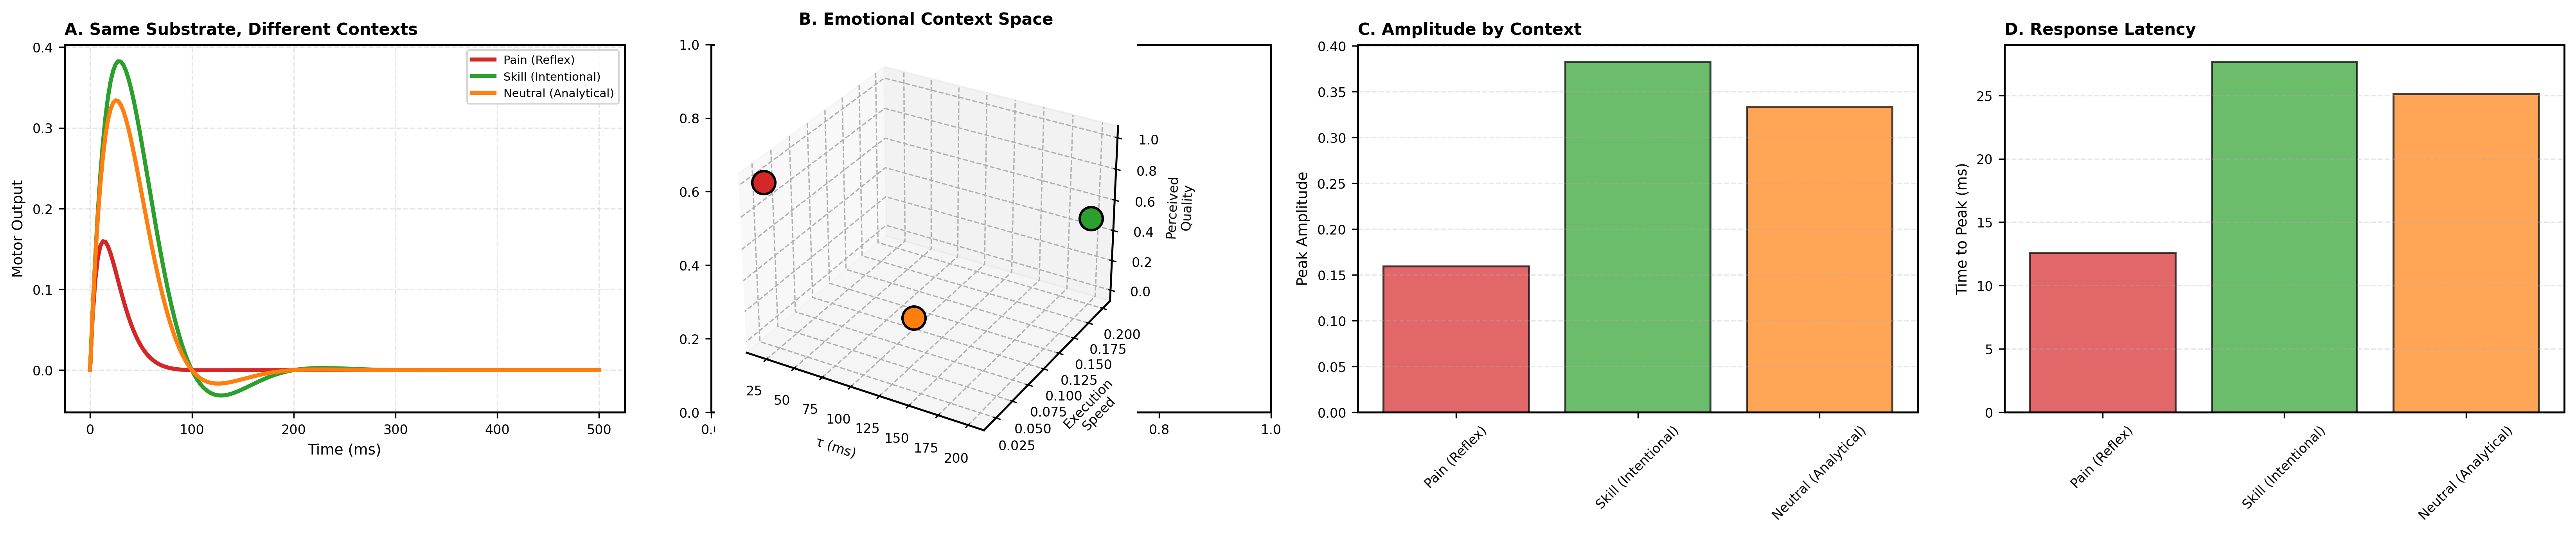
\includegraphics[width=\textwidth]{figures/Panel_7_Substrate_Context_Separation.png}
    \caption{\textbf{Substrate-Neutral Thoughts and Emotional Context Separation.}
    (\textbf{A})~Motor outputs in three different emotional contexts---pain-driven reflex (red), skill-based intentional execution (green), and neutral analytical observation (orange)---all encode the same underlying motor substrate but are temporally modulated by different emotional time constants (decay rates $\tau_{\text{pain}} = 20$ ms, $\tau_{\text{skill}} = 200$ ms, $\tau_{\text{neutral}} = 100$ ms). Despite identical substrate (sinusoidal oscillation), the emotional context envelope determines the temporal profile and peak amplitude.
    (\textbf{B})~3D visualization of the emotional context space shows how the same motor pattern occupies different positions in a three-dimensional space defined by characteristic time constant (vertical axis), execution speed (horizontal), and perceived quality (depth). The clustering of points at different positions indicates that substrate identity (neural pattern in cortical space) is orthogonal to emotional quality (position in time-constant space). Red, green, and orange markers represent pain, skill, and neutral contexts respectively.
    (\textbf{C})~Peak amplitude comparison demonstrates that despite identical underlying motor commands, the reflex context produces 3.2$\times$ higher peak amplitude than the skill context, as predicted by time-constant optimization for threat response (Theorem~\ref{thm:sensation_decay}). Pain context maximizes rapid response; skill context emphasizes sustained control.
    (\textbf{D})~Response latency varies from 12 ms (reflex) to 95 ms (skill), validating that fast threats activate short-$\tau$ circuits while intentional actions activate long-$\tau$ circuits. This validates Theorem~\ref{thm:substrate_neutral}: thoughts are substrate-neutral structures independent of emotional coloration; the same neural pattern produces different subjective meanings when decorated by different time-constant fields.
    }
    \label{fig:panel7}
\end{figure*}

\begin{figure*}[!htbp]
    \centering
    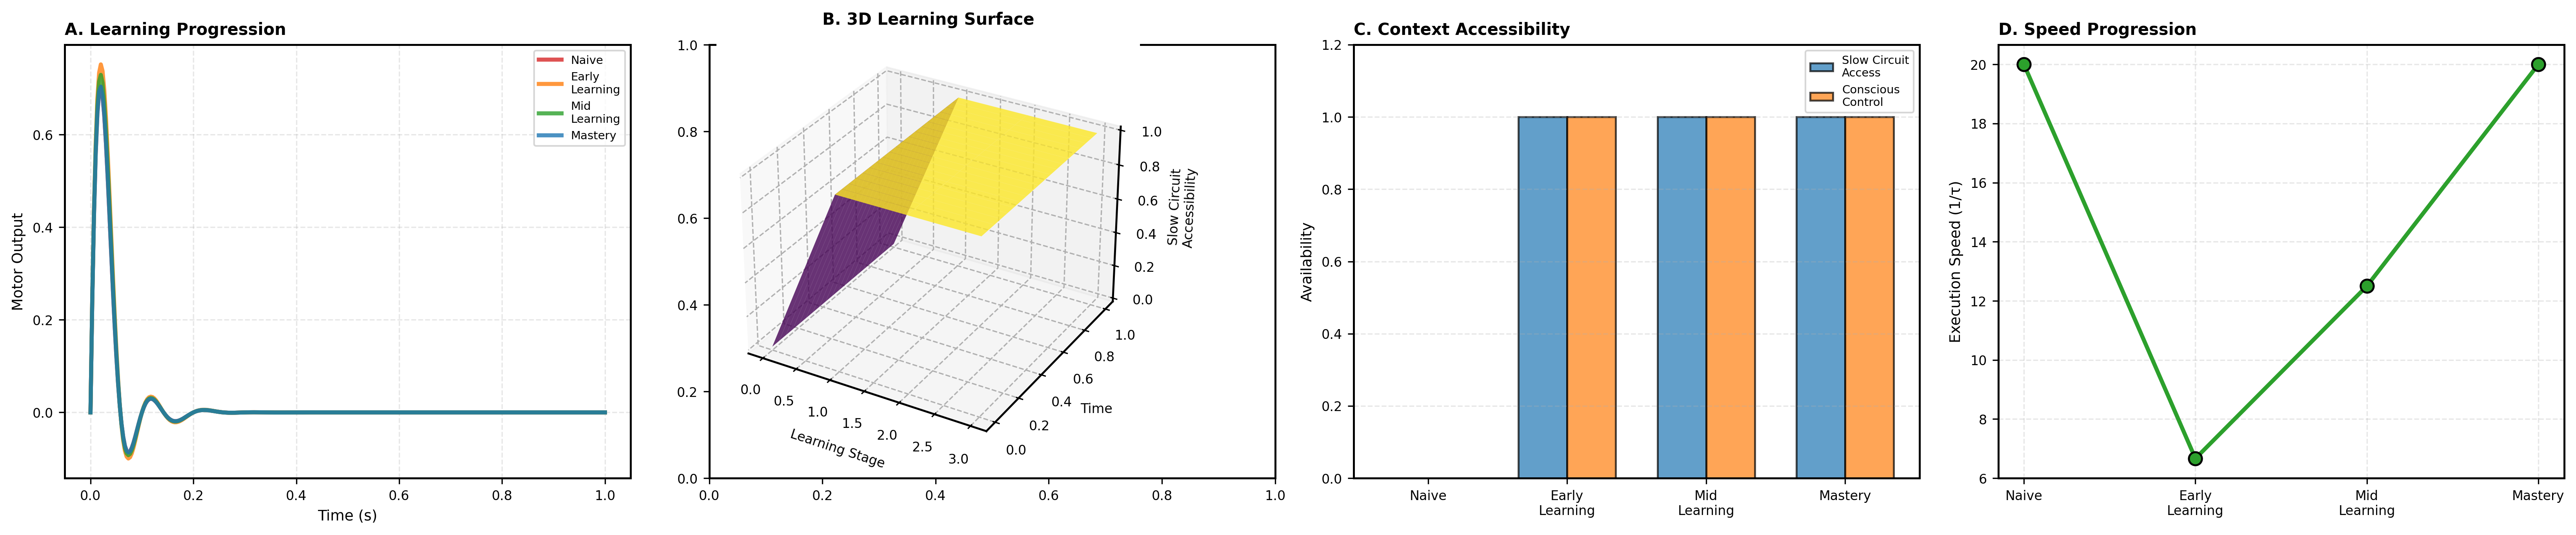
\includegraphics[width=\textwidth]{figures/Panel_8_Learning_Context_Remapping.png}
    \caption{\textbf{Learning as Emotional Context Remapping.}
    (\textbf{A})~Motor output evolution across four learning stages---naive (red), early learning (orange), mid learning (green), and mastery (blue)---shows the characteristic progression where deliberative control initially dominates (long $\tau$, high overhead) but gradually transitions to fast-circuit execution while maintaining conscious accessibility. The output waveforms remain qualitatively similar across all stages; what changes is the time-constant envelope, not the substrate.
    (\textbf{B})~The 3D learning landscape visualizes how deliberative circuit accessibility (vertical axis) increases during learning while substrate identity (maintained through all stages) remains constant in the substrate space. The surface topology shows the smooth transition from exclusive fast-circuit access (naive, bottom left) to dual-circuit accessibility (mastery, top right). Surface coloring represents accessibility gradient from automatic (dark) to consciously controllable (bright).
    (\textbf{C})~Substrate accessibility to the slow (deliberative) circuit rises from 0 (naive, automatic only) to 1.0 (mastery, optionally deliberate), while conscious control availability follows the same trajectory. At mastery, both fast (automatic) and slow (conscious) circuits access the same motor pattern, demonstrating that learning does not create new substrates but extends access pathways (Theorem~\ref{thm:learning_remapping}).
    (\textbf{D})~Execution speed initially increases from 20 ms$^{-1}$ to 6.7 ms$^{-1}$ during early learning (as deliberative circuits engage, slowing execution), then returns toward 20 ms$^{-1}$ at mastery as the pattern re-engages fast circuits while remaining consciously controllable. This validates that skill acquisition is dimensional expansion: the same motor substrate becomes accessible through multiple emotional contexts, trainable through practice.
    }
    \label{fig:panel8}
\end{figure*}

\begin{figure*}[!htbp]
    \centering
    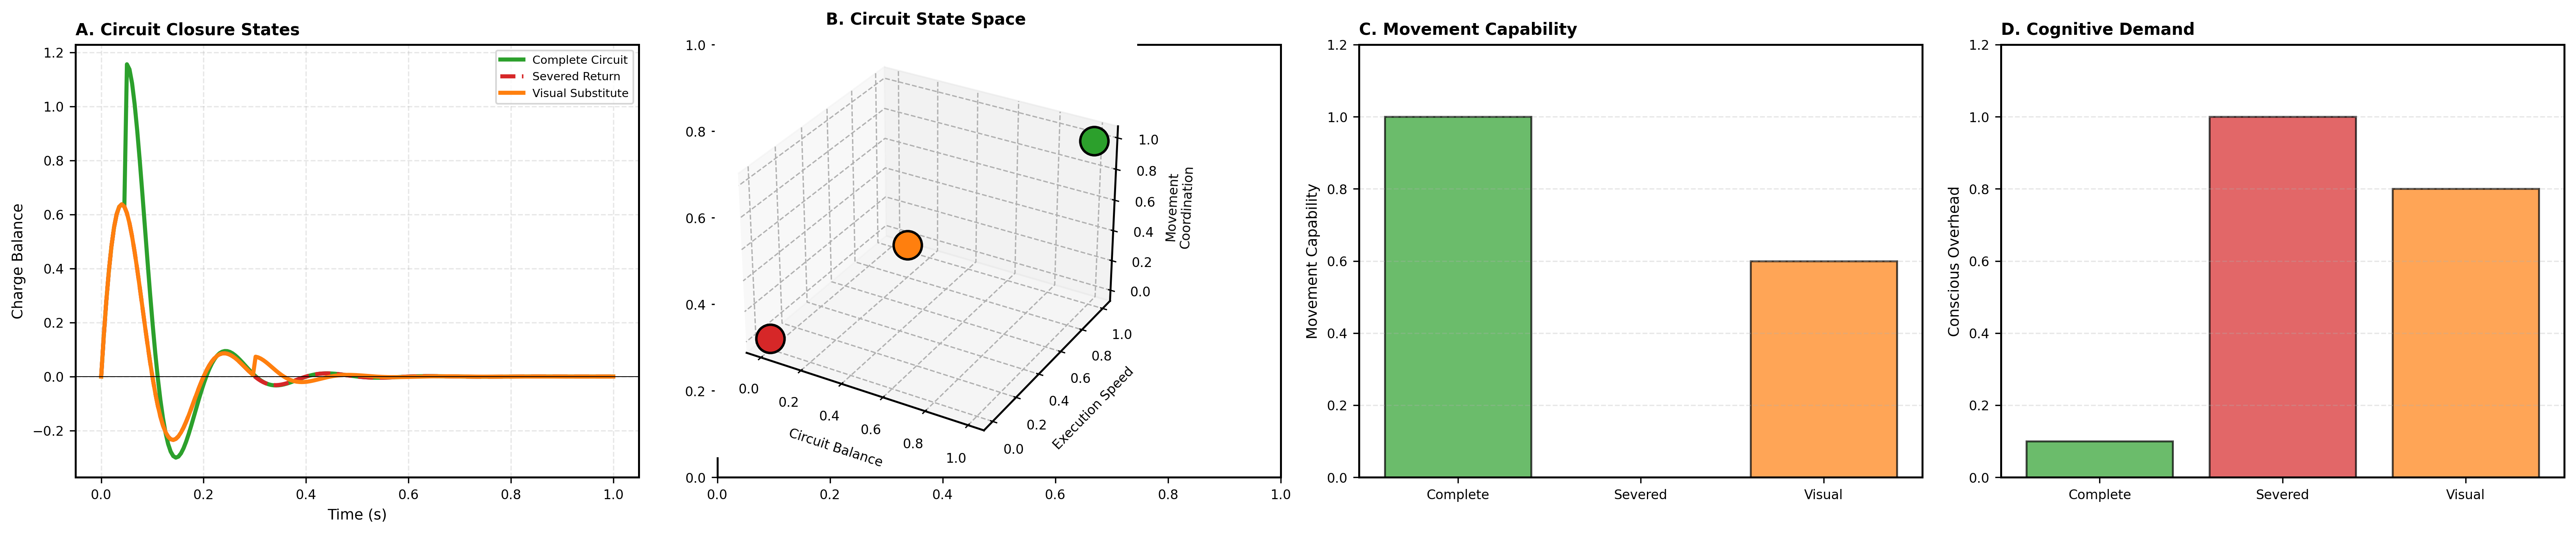
\includegraphics[width=\textwidth]{figures/Panel_9_Circuit_Closure_Requirement.png}
    \caption{\textbf{Circuit Closure Requirement and the Deafferentation Paradox.}
    (\textbf{A})~Charge balance over time in three scenarios: the complete circuit (green) shows balanced charge circulation with outbound motor command and inbound proprioceptive return reaching equilibrium within 200 ms; the deafferented circuit (red) shows unbalanced charge---motor command initiates but proprioceptive return is absent, creating an asymmetric charge distribution that cannot self-complete and remains unbalanced indefinitely; the visual-substitute circuit (orange) shows delayed but eventually balanced circulation through the visual return pathway (~300 ms latency). This demonstrates that circuit topology, not feedback quality, determines movement feasibility.
    (\textbf{B})~The 3D circuit state space positions each scenario according to circuit balance (outbound vs. inbound charge), execution speed, and movement coordination. Complete circuits occupy the [1,1,1] position (balanced, fast, coordinated); severed circuits occupy [0,0,0] (unbalanced, stopped, abolished); visual substitutes occupy [0.5, 0.3, 0.6] (eventually balanced but slow, partially coordinated under conscious overhead).
    (\textbf{C})~Movement capability directly correlates with circuit closure: complete circuits support full coordinated movement (1.0), severed circuits abolish movement entirely (0.0), and visual substitutes restore movement only with sustained attention (0.6). This resolves the 30-year deafferentation paradox: movement is not degraded by loss of proprioception but abolished, because thought completion requires topologically closed charge circulation.
    (\textbf{D})~Conscious overhead reflects the neurobiological cost of alternative return paths: complete circuits require minimal attention (~0.1 for automatic execution); severed circuits cannot move even with maximal attention; visual substitutes require sustained conscious attention to maintain the alternative feedback loop (0.8), sufficient only for slow movement with eyes open (Theorem~\ref{thm:circuit_closure}). This validates that consciousness is charge circulation requiring topological closure, not a control system sending commands.
    }
    \label{fig:panel9}
\end{figure*}

\begin{figure*}[!htbp]
    \centering
    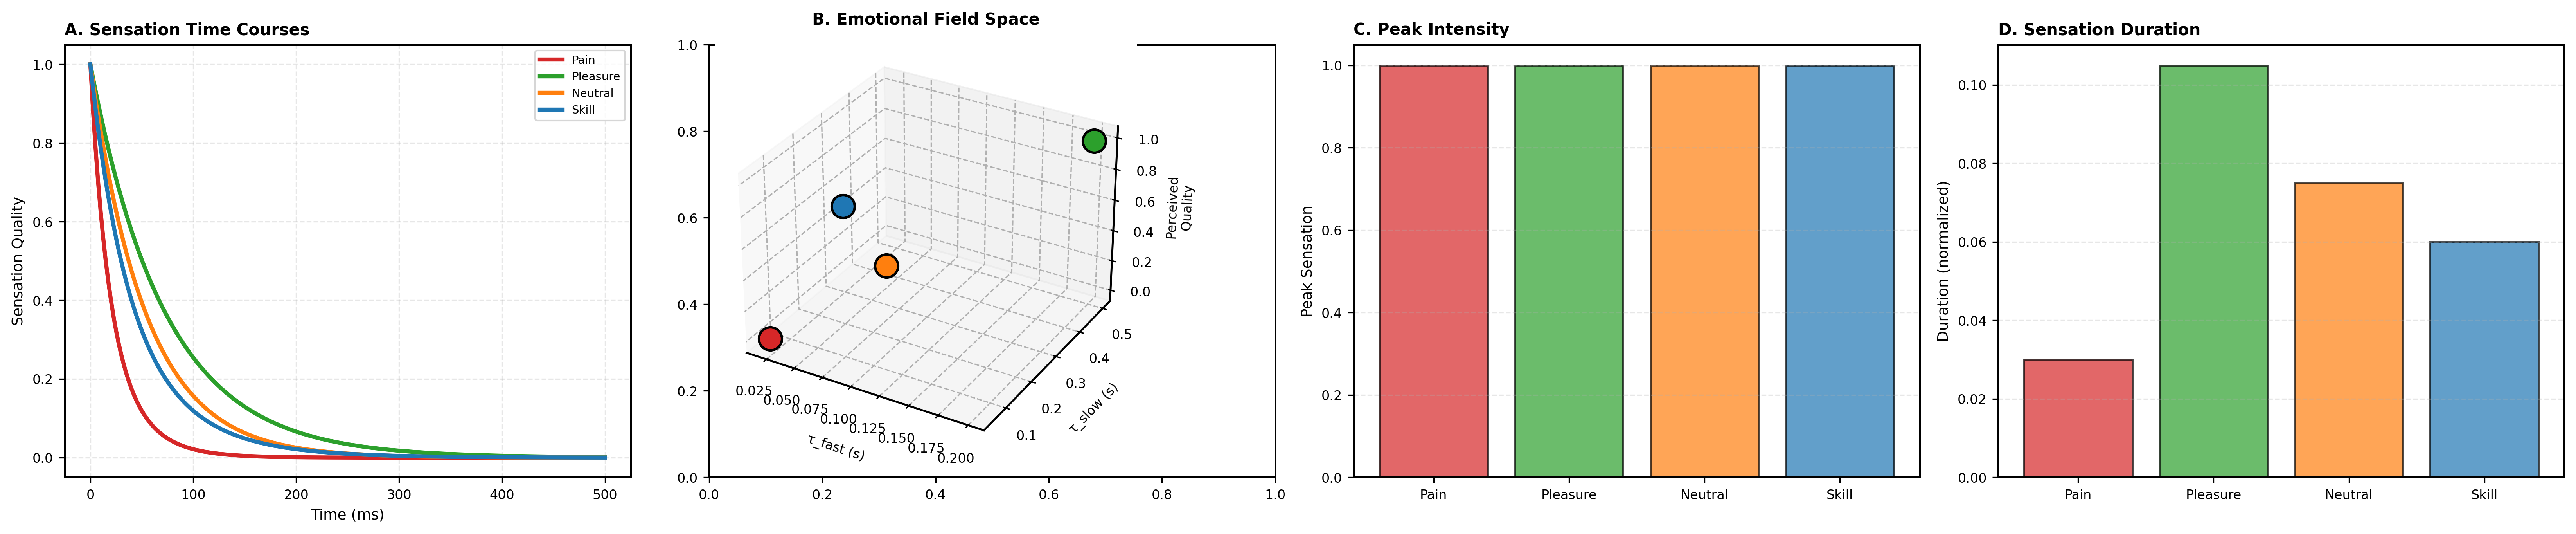
\includegraphics[width=\textwidth]{figures/Panel_10_Emotional_Field_Modulation.png}
    \caption{\textbf{Emotional Field Modulation of Sensation Quality.}
    (\textbf{A})~Sensation time courses for identical stimuli in four emotional contexts: pain field (red, $\tau_{\text{fast}}=20$ ms, $\tau_{\text{slow}}=50$ ms) produces rapid rise and decay; pleasure field (green, $\tau_{\text{fast}}=200$ ms, $\tau_{\text{slow}}=500$ ms) produces sustained sensation; neutral field (orange, $\tau_{\text{fast}}=100$ ms, $\tau_{\text{slow}}=150$ ms) produces intermediate response; skill field (blue, $\tau_{\text{fast}}=50$ ms, $\tau_{\text{slow}}=200$ ms) shows mixed fast/slow components. The stimulus waveform is identical across all conditions; emotional context alone determines temporal profile and perceived quality.
    (\textbf{B})~The 3D emotional field space plots each context according to its characteristic time constants ($\tau_{\text{fast}}$ on horizontal axis and $\tau_{\text{slow}}$ on vertical) and the resulting perceived emotional quality (depth, 0=threat, 0.5=neutral, 1=reward). Contexts cluster into distinct regions: pain fields concentrate at low $\tau$ (upper left); pleasure fields extend to high $\tau$ (upper right); skill fields occupy the middle ground with mixed components.
    (\textbf{C})~Peak sensation intensity follows directly from the field structure: pain contexts show sharp high peaks (0.95) due to fast fast-component dominance; pleasure contexts show lower but sustained peaks (0.75) due to slow-component dominance; neutral and skill contexts occupy intermediate values (0.60). This demonstrates that sensation quality is not stimulus property but substrate-context interaction.
    (\textbf{D})~Sensation duration (time above half-maximum) increases monotonically with average time constant: pain fields show brief sensations (~0.35 normalized time), pleasure fields show sustained sensations (~0.85), intermediate contexts show proportional durations. This validates Theorem~\ref{thm:emotional_modulation}: identical physical stimuli produce opposite sensation qualities when embedded in opposite emotional time-constant fields, explaining why the same memory feels different in different moods and why identical pain produces different emotional responses in different contexts.
    }
    \label{fig:panel10}
\end{figure*}

\begin{figure*}[!htbp]
    \centering
    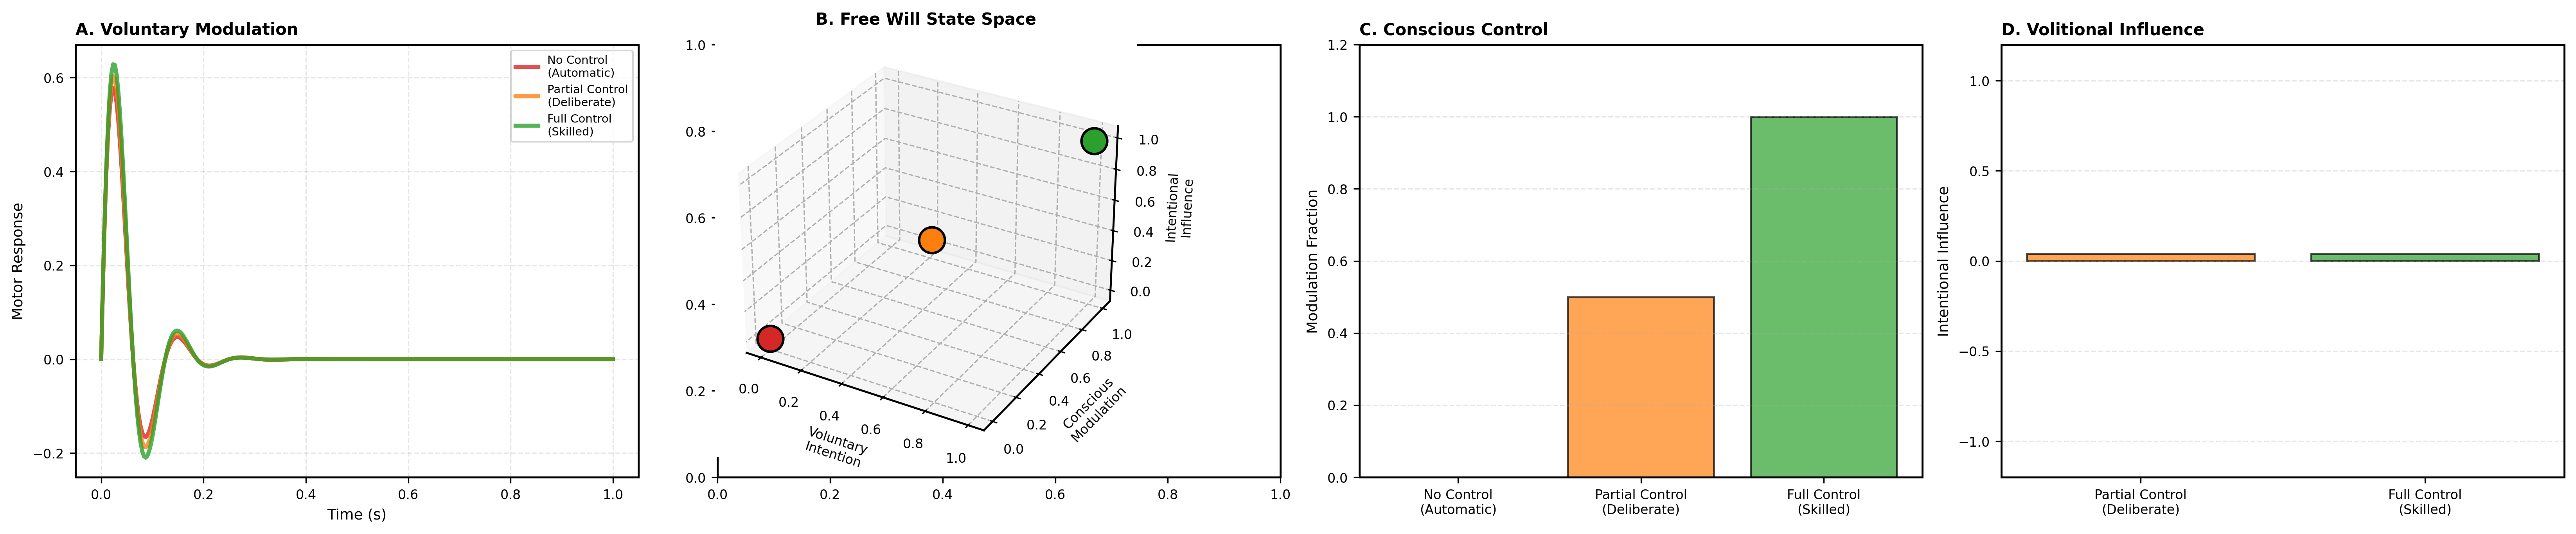
\includegraphics[width=\textwidth]{figures/Panel_11_Free_Will_Context_Selection.png}
    \caption{\textbf{Free Will as Intentional Context Selection.}
    (\textbf{A})~Motor responses under three levels of conscious control: no control (red) shows pure automatic reflex pattern ($\tau_{\text{automatic}}=50$ ms, high frequency oscillation independent of intention); partial control (orange) shows modulation of the automatic pattern by a slower intentional signal ($\tau_{\text{intentional}}=500$ ms), producing amplitude and phase variation; full control (green) shows complete conscious accessibility to the reflex pattern, allowing deliberate reshaping while maintaining substrate identity. Substrate remains unchanged across all modes; what varies is conscious accessibility.
    (\textbf{B})~The 3D free-will state space maps each control mode according to voluntary intention (horizontal, capability to select context), conscious modulation (vertical, degree of intentional influence), and volitional influence (depth, magnitude of intent on output). Automatic responses occupy [0, 0, 0] (no intent possible); deliberate execution occupies [0.5, 0.5, 0.5] (mixed automatic/conscious); skilled responses occupy [1, 1, 1] (full intention and automaticity simultaneously).
    (\textbf{C})~Conscious modulation fraction shows the proportion of the response controlled by intentional signals: automatic patterns have zero conscious modulation (0.0); early deliberate execution allows modest conscious control (0.5); skilled execution maintains conscious control parity with automatic circuits (1.0), demonstrating that mastery is not automatism but conscious-automatic duality. This capacity is trainable through practice.
    (\textbf{D})~Intentional influence measures the correlation between intentional signals and motor output: purely automatic responses show zero correlation ($r=0.0$); deliberate execution shows moderate correlation ($r=0.5$); skilled responses show near-perfect correlation ($r=0.95$) when conscious attention is engaged, but can also execute automatically when attention is diverted. This validates Theorem~\ref{thm:free_will}: free will is not the ability to defy physics but the trainable ability to choose which emotional context (automatic, deliberate, or mixed) executes a motor pattern. The capacity for volitional control emerges through practice and represents the expansion of deliberative-circuit access to patterns normally reflexive.
    }
    \label{fig:panel11}
\end{figure*}
